\begin{figure}[ht]
    \centering
    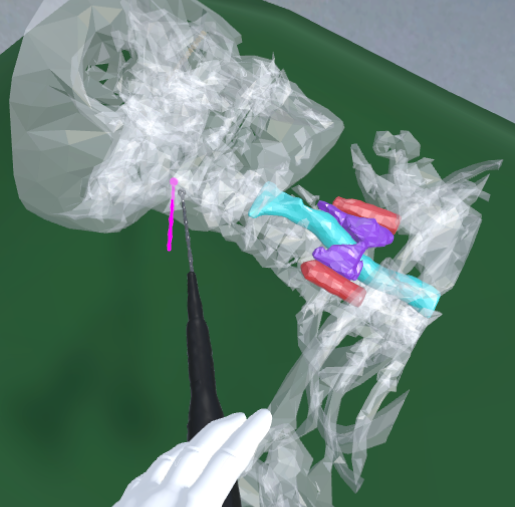
\includegraphics[width=200px]{images/implementation/features/procedures/drilling.png}
    \caption{\label{fig::FeatureDrilling} Drilling Procedure}
\end{figure}

The drilling operation is performed by picking up the bonesaw (Figure \ref{fig::FeatureDrilling}).
In total, there are fifteen attachments which can be used for the drilling procedure.

\begin{figure}[ht]
    \centering
    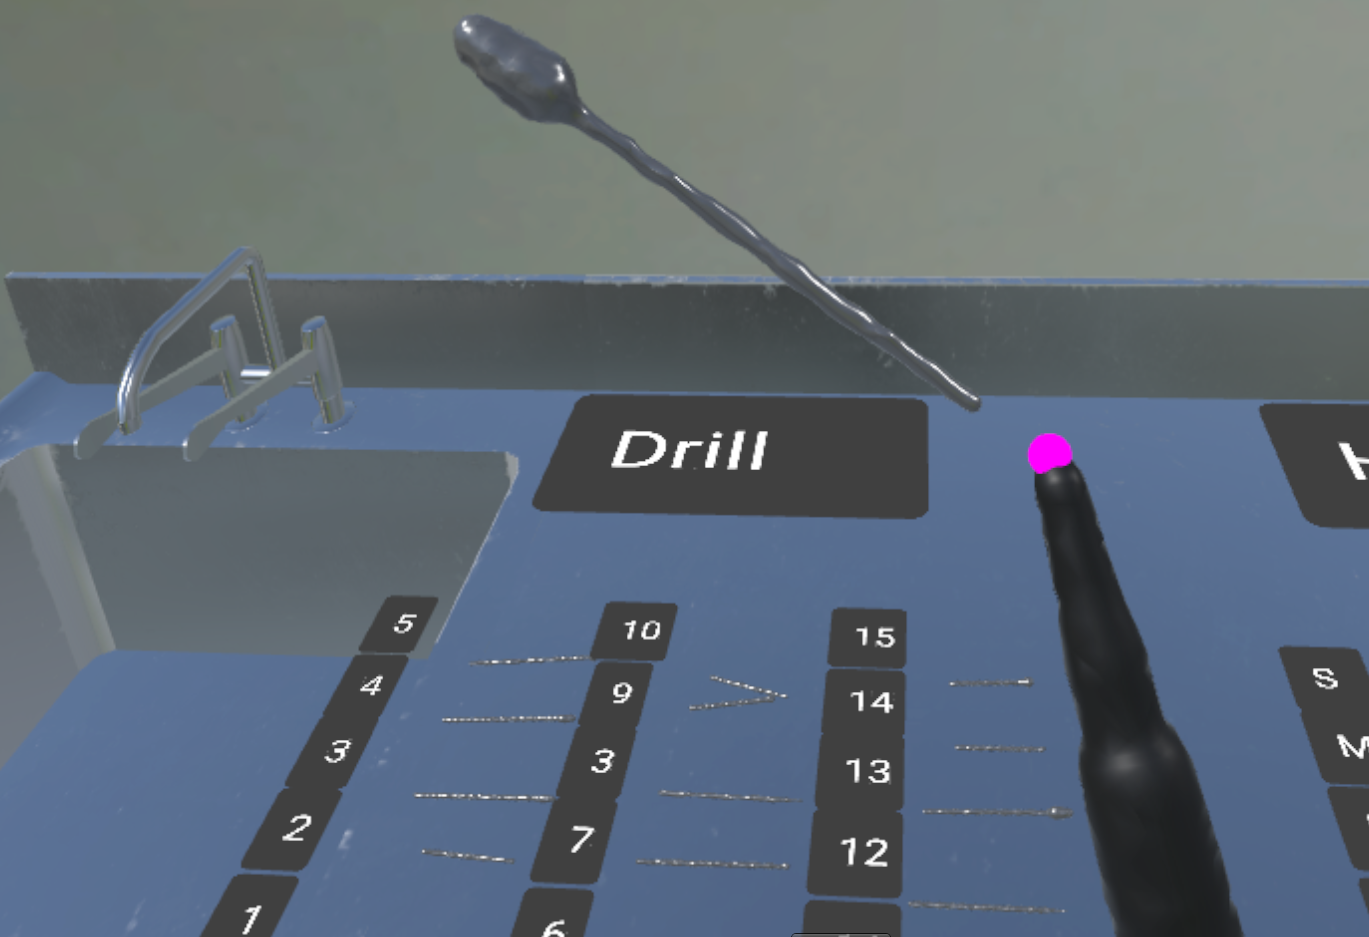
\includegraphics[width=200px]{images/implementation/features/procedures/drilling_attachment.png}
    \caption{\label{fig::FeatureDrillingAttachments} Attaching an Attachment to the Surgical Drill}
\end{figure}

Attachments get attached to the virtual drill be holding the indicate button of the controller in which hand the drill is currently located and moving the attachment to the indicated circle \ref{fig::FeatureDrillingAttachments}.
To perform the procedure, an attachment must be currently attached to the virtual drill.
Performing the virtual procedure will create a copy of the current attachment with a different material to indicate that is is part of the project case.
To increase performance in the AR and VR workflow, since the AR hardware is not as capable as high end computers which are needed for VR, the resolution of the attachments has been decreased at the processing step as described at the start of this section.